
\begin{comment}
PIECEWISE SMOOTH SURFACE (x==0&&y==0)?0:f(x,y) means at (0,0) the function equals 0 else it equals f(x,y)

\begin{figure}
\centering
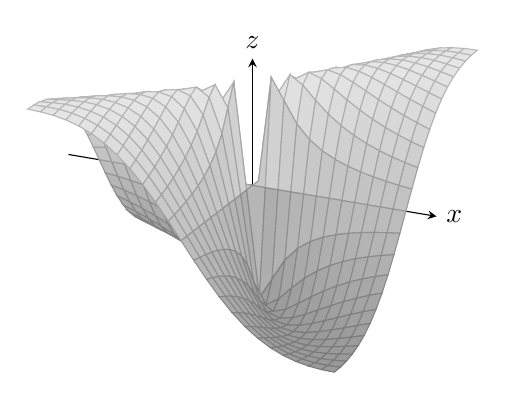
\begin{tikzpicture}[declare function={f(\x,\y)=2*\x*\y/((\x)^2+(\y)^2);}]
  \begin{axis}[axis lines=center,colormap={}{gray(0.2cm)=(0.6);gray(1cm)=(0.9);},enlargelimits=true,xlabel={$x$},ylabel={$y$},zlabel={$z$},hide y axis,xlabel style={anchor={west}},zlabel style={anchor=south},xtick={\empty},ytick={\empty},ztick={\empty}]
    \addplot3[surf] { (x==0&&y==0) ?0 : f(x,y) } ;
  \end{axis}
\end{tikzpicture}
\end{figure}
\end{comment}

\begin{figure}
\centering
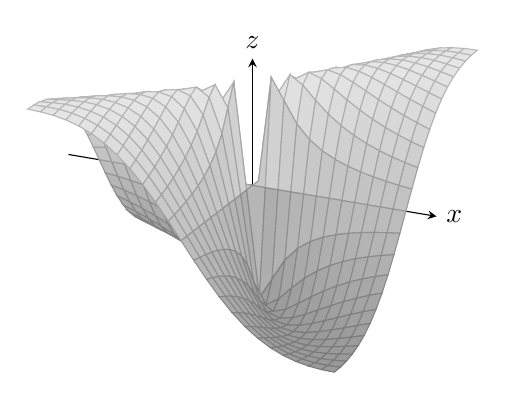
\begin{tikzpicture}[declare function={f(\x,\y)=2*\x*\y/((\x)^2+(\y)^2);}]
  \begin{axis}[axis lines=center,colormap={}{gray(0.2cm)=(0.6);gray(1cm)=(0.9);},enlargelimits=true,xlabel={$x$},ylabel={$y$},zlabel={$z$},hide y axis,xlabel style={anchor={west}},zlabel style={anchor=south},xtick={\empty},ytick={\empty},ztick={\empty}]
    \addplot3[surf] { (x==0&&y==0) ?0 : f(x,y) } ;
  \end{axis}
\end{tikzpicture}
\end{figure}

